\newpage
\section{Diskussion}
\label{sec:Diskussion}
Zuallererst fällt auf, dass die experimentellen Werte kleiner sind als die theoretischen Werte.
Insgesamt sind die Abweichung von der Theorie aber geringfügig. So ist das theoretisch bestimmte Trägheitsmoment
des Zylinders lediglich um $2{,}74\%$ größer als das experimentell bestimmte. Für die Kugel ist das theoretische bestimmte 
Trägheitsmoment $7{,}41\%$ größer.\\
Für die Puppe in der ersten Körperhaltung ist das experimentelle Trägheitsmoment um $1.358{,}41 \%$ größer als das theoretische Trägheitsmoment.
Für die Puppe in der zweiten Körperhaltung ist das experimentelle Trägheitsmoment um  größer als das theoretische Trägheitsmoment.\\
Messfehler können durch das Wiegen der Massen, Ablesefehler der Schieblehre oder des Federkraftmessers entstanden sein. Weiterhin sind zwar die
Schwingungsdauern durch das Messen mehrer Schwingungen vermutlich genauer als durch das Messen genau einer Schwingung, aber dennoch wird die Reaktionszeit beim 
Stoppen der Uhr für größere Messfehler gesorgt haben.\\
Weiterhin geht die Drehachse der Puppe nicht durch die angenommene theoretische angenommene Drehachse und die Annäherung der Puppe der Zylinder ist auch sehr grob,
so dass sich dadurch die großen Abweichungen erklären lassen.\\
Insgesamt lässt sich fest halten, dass die Theorie sich zumindest für geometrisch sehr einfache Körper wie eine Kugel oder einen Zylinder bestätigen lässt.

\newpage

\section{Messwerte}
\begin{figure}
    \centering
    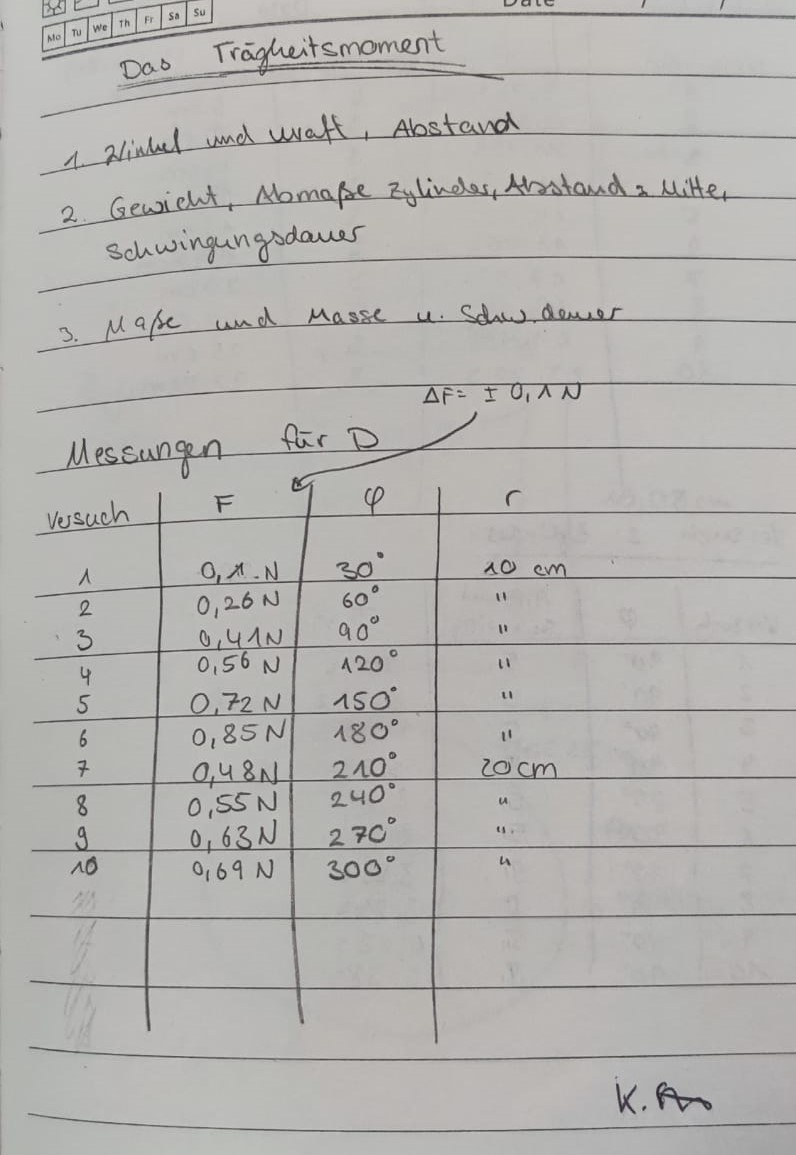
\includegraphics[width=0.7\textwidth]{index.jpg}
    \caption{Messdaten Teil 1}
    \label{fig:M1}
  \end{figure}

\begin{figure}
    \centering
    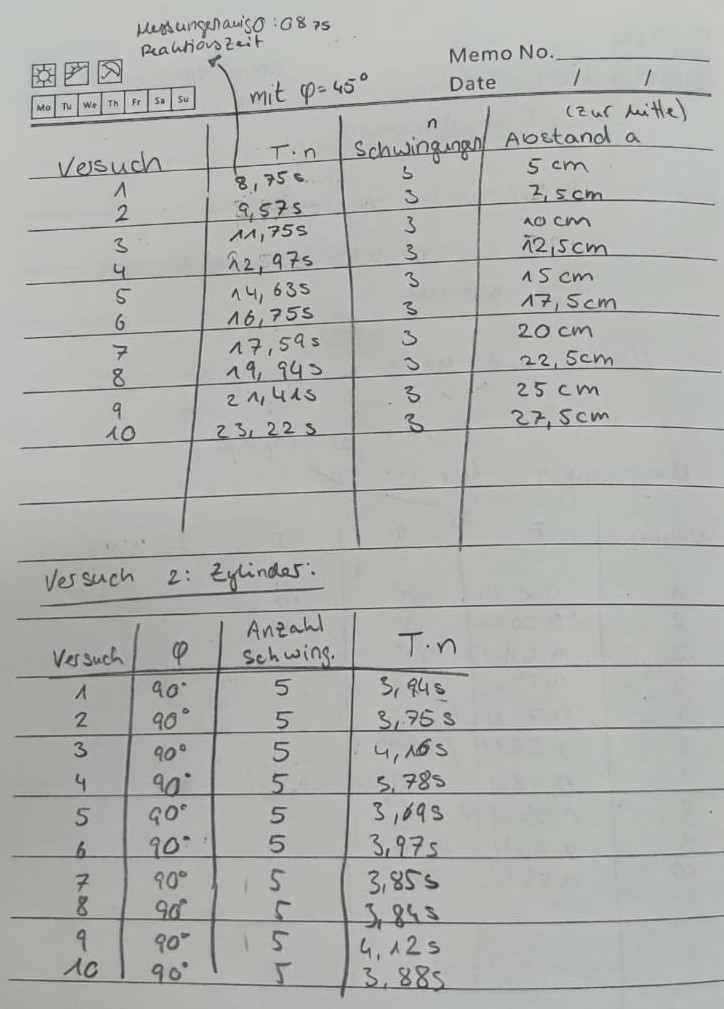
\includegraphics[width=0.7\textwidth]{index2.jpg}
    \caption{Messdaten Teil 2}
    \label{fig:M1}
\end{figure}

\begin{figure}
  \centering
  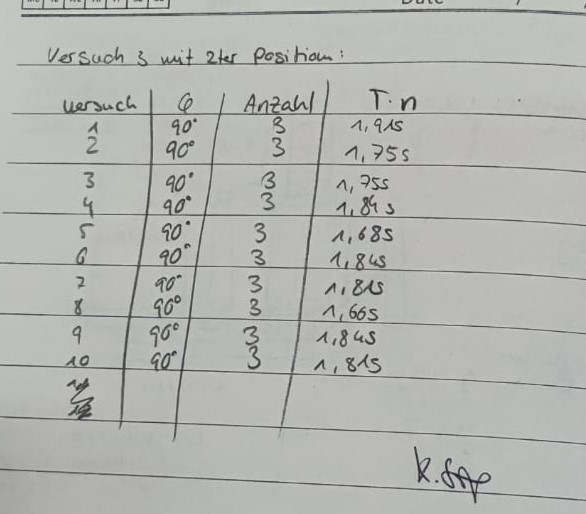
\includegraphics[width=0.7\textwidth]{index3.jpg}
  \caption{Messdaten Teil 3}
  \label{fig:M1}
\end{figure}
\begin{figure}
  \centering
  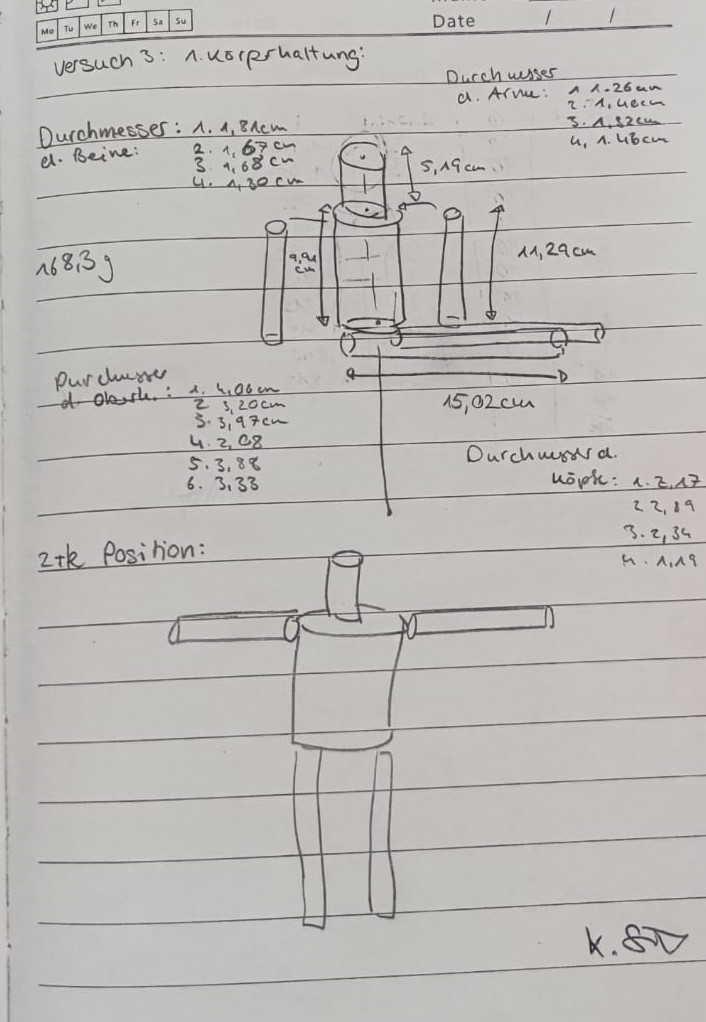
\includegraphics[width=0.7\textwidth]{index4.jpg}
  \caption{Messdaten Teil 4}
  \label{fig:M1}
\end{figure}
\begin{figure}
  \centering
  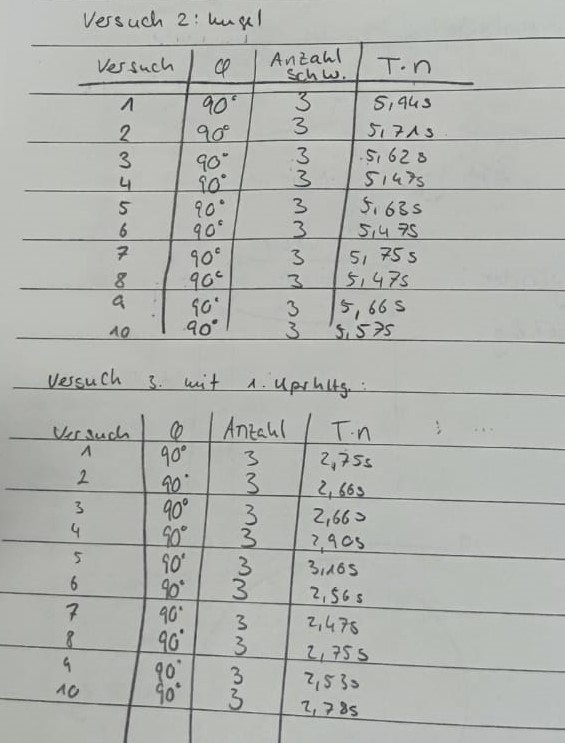
\includegraphics[width=0.7\textwidth]{index5.jpg}
  \caption{Messdaten Teil 5}
  \label{fig:M1}
\end{figure}

\begin{figure}
  \centering
  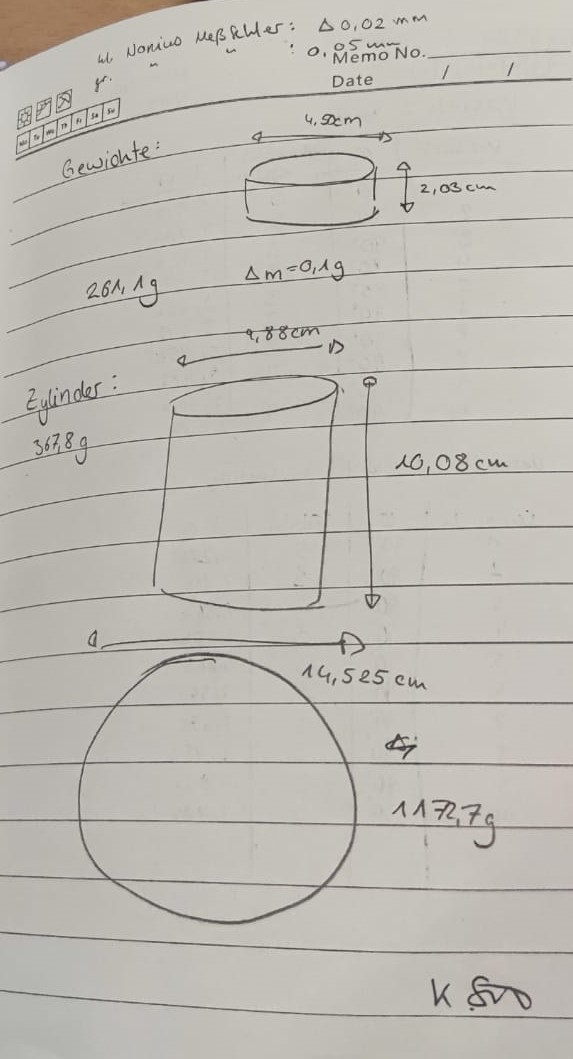
\includegraphics[width=0.7\textwidth]{index6.jpg}
  \caption{Messdaten Teil 6}
  \label{fig:M1}
\end{figure}